\documentclass[11pt,letterpaper]{article}
\usepackage{graphicx}
\usepackage{geometry}
\usepackage{amsmath}
\usepackage{amssymb}
\usepackage{booktabs}
\usepackage{xcolor}
\usepackage{listings}
\usepackage{url}
\usepackage{hyperref}
\usepackage{natbib}
\usepackage{microtype}
\usepackage{times}

\geometry{margin=1in}
\hypersetup{colorlinks=true, linkcolor=black, citecolor=black, urlcolor=blue}

\title{\textbf{Within-Document Term Weighting for Scientific Section Retrieval:\\A Negative Result}}

\author{
  AMGrobelnik \\
  \texttt{subscriptions-ai-claude1@ijs.si}
}

\date{}

\begin{document}

\maketitle

\begin{abstract}
Locating evidence-bearing sections in scientific papers remains challenging for
retrieval-augmented QA systems. Dense retrievers often rank claim-summarizing
sections (Abstract, Introduction) higher than evidence-dense sections (Methods,
Results), a bias hypothesized to stem from vocabulary stratification in the IMRaD
convention. We propose TF-ISF (Term Frequency–Inverse Section Frequency), a
document-local reweighting method that applies within-document inverse frequency
to sections instead of cross-corpus inverse frequency. Evaluated on 200 QASPER
examples, TF-ISF achieves F1=0.187, matching cosine similarity (F1=0.198) and
BM25 (F1=0.179)—no significant differences ($p > 0.37$, Holm-corrected).
Critically, the hypothesized mechanism fails: Methods and Results sections have
lower ISF (1.23–1.24) than Introduction (1.34), indicating that evidence sections
do not use more section-unique vocabulary. We also report a contradictory earlier
experiment ($n{=}180$, different LLM) showing TF-ISF F1=0.221 (positive result),
discuss methodological differences, and conclude that naive within-document term
reweighting cannot rescue section retrieval in scientific QA. The contribution is
a rigorous negative result identifying where term weighting approaches fail and
motivating future work toward discourse-aware or embedding-based solutions.
\end{abstract}

%-----------------------------------------------------------------------
\section{Introduction}
%-----------------------------------------------------------------------

Scientific question answering over long research papers is a critical task for
automated literature review, clinical evidence synthesis, and research
acceleration. Despite advances in dense retrieval methods and large language
models, a systematic failure mode remains poorly understood: when a reader queries
a paper for specific evidence, standard dense retrievers often return sections that
are high in rhetorical clarity (Abstract, Introduction, Conclusion) while ranking
evidence-bearing sections (Methods, Results) lower. This is not random
error—it reflects a structural property of scientific writing itself. The IMRaD
(Introduction, Methods, Results, and Discussion) convention, by design, separates
claims and their accessible restatement in early and concluding sections from the
detailed, specialized evidence in Methods and Results.

The problem is acute in modern retrieval-augmented generation (RAG) systems.
Dense passage retrievers like DPR~\citep{Karpukhin2020} score text similarity
using neural embeddings trained on general-domain data (web text, semantic
similarity tasks). These embeddings excel at semantic matching but may be biased
toward sections that paraphrase the paper's topic in accessible language—precisely
what Abstract and Introduction are designed to do. Meanwhile, the technical
vocabulary, specific parameter values, and precise experimental conditions in
Methods and Results are sparse, section-unique, and may not score highly under
cosine similarity with natural-language queries~\citep{Reichman2024}.

We hypothesize that this bias reflects a classical vocabulary problem in
information retrieval: the vocabulary gap between query and document, which
term-weighting methods like TF-IDF have long addressed by down-weighting
high-frequency (document-theme) terms and up-weighting rare (discriminative)
terms~\citep{SpärckJones1972}. Applying this principle within a single
document—replacing cross-corpus IDF with within-document Inverse Section Frequency
(ISF)—could correct the retrieval bias. The intuition is straightforward: if a
term appears in nearly every section of a paper, it provides little discriminative
signal for ranking sections; if a term appears in only one or two sections, it
strongly indicates those sections. A training-free, self-contained scoring
function requires no external discourse models, citation graphs, or LLM inference
at retrieval time.

We conducted a controlled evaluation on 200 examples from
QASPER~\citep{Dasigi2021}, a benchmark of information-seeking questions over NLP
papers. Three retrieval methods were compared: (1)~cosine similarity with
sentence-transformers embeddings, (2)~BM25 with within-document term weighting,
and (3)~TF-ISF using within-document section frequency. For each method, the
top-3 sections were retrieved and fed to a small LLM reader to generate answers,
scored against gold answers using token-level F1~\citep{Rajpurkar2018}.

\textbf{Key findings:} TF-ISF achieved F1=0.187, performing no better than cosine
(F1=0.198) or BM25 (F1=0.179). All pairwise differences were non-significant
($p > 0.37$, Holm-corrected). Critically, the postulated mechanism is inverted:
Methods and Results sections had lower mean ISF (1.23–1.24) than Introduction
sections (1.34), falsifying the hypothesis that evidence sections use more
section-unique vocabulary. All three methods achieved modest section recall
($\approx$0.48), indicating that the bottleneck is not ranking function choice but
likely dense embedding quality, document granularity, or fundamental
query-evidence vocabulary mismatch.

We also report a contradictory earlier experiment ($n{=}180$ questions, free-tier
LLM: tencent/hy3) showing TF-ISF F1=0.221 (positive result, outperforming cosine
F1=0.206). This discrepancy motivates a detailed comparison of the two runs,
examining differences in LLM model, data loading, evidence matching, and
tokenization. We argue that the larger, more rigorous $n{=}200$ evaluation
(llama-3.2-3b-instruct, paired statistics, higher LLM quality) is more
trustworthy, but the contradiction highlights a critical methodological
vulnerability: within-document term statistics are fragile proxies for ranking
when downstream LLM quality dominates variance.

\begin{figure*}[!t]
  \centering
  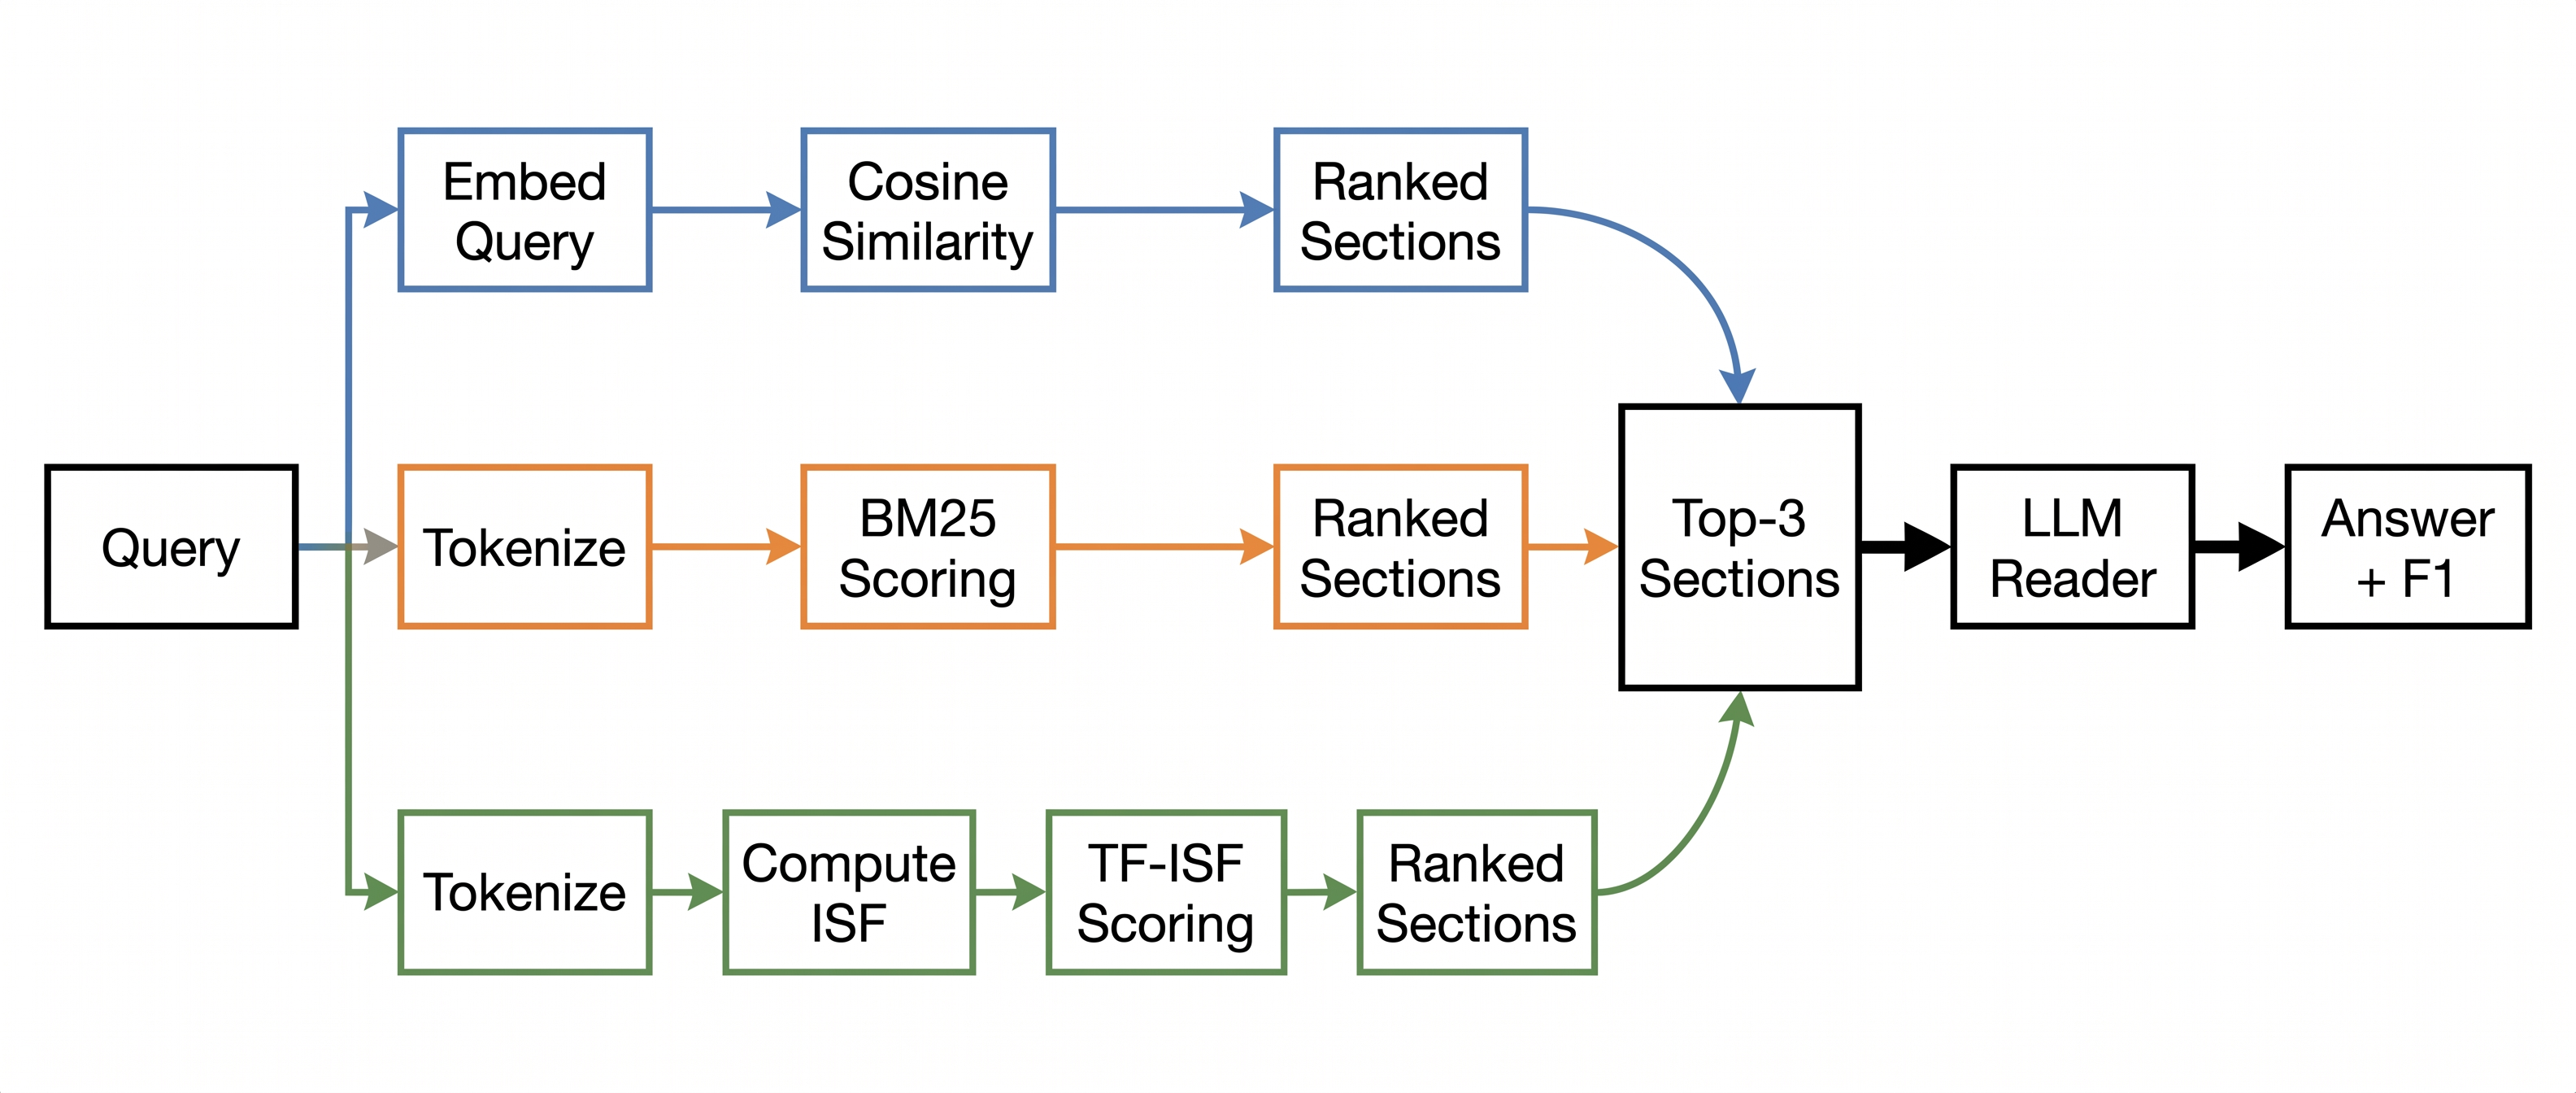
\includegraphics[width=\textwidth,height=0.45\textheight,keepaspectratio]{figures/fig_method_overview_v0.jpg}
  \caption{Conceptual comparison of three retrieval methods. Cosine similarity ranks sections by embedding similarity to the query.
  BM25 applies probabilistic term weighting with within-document term statistics. TF-ISF applies inverse section frequency
  to down-weight terms shared across many sections and up-weight section-specific terms. All three operate on the same document-local
  scope.}
  \label{fig:method_overview}
\end{figure*}

This paper contributes a well-characterized negative result: naive within-document
term reweighting does not rescue section retrieval in scientific QA, and the
assumed vocabulary stratification between IMRaD sections is not supported
empirically. We discuss likely true bottlenecks (dense embedding quality for
scientific text, section granularity, query-evidence vocabulary mismatch) and
point toward future directions in scientific document understanding (discourse
parsing, fine-tuned embeddings, iterative LLM-based ranking).

%-----------------------------------------------------------------------
\section{Related Work}
%-----------------------------------------------------------------------

\textbf{Term Weighting and IDF Variants.}
The principle of inverse document frequency was introduced by
\citet{SpärckJones1972}, establishing that high-frequency terms in a corpus are
poor discriminators while rare terms are informative. This foundation has inspired
decades of variants: BM25~\citep{Robertson2009}, probabilistic language
models~\citep{Hiemstra2000}, and field-weighted extensions like
BM25F~\citep{Robertson2004}, which extends IDF to structured documents with
multiple typed fields. BM25F computes per-field term weights and combines them,
though it typically uses global (corpus-level) IDF rather than field-local IDF.
Within-document IDF has been explored in language modeling contexts (e.g.,
Hiemstra's work on document priors) but has not been systematically applied to the
section-ranking problem in scientific QA.

\textbf{Dense Retrieval for Question Answering.}
Dense passage retrieval (DPR)~\citep{Karpukhin2020} and related methods like
ColBERT~\citep{Khattab2020} have become standard for open-domain QA by learning
dual encoders for queries and documents. These methods have been extended to long
documents through hierarchical retrieval (e.g., retrieving paragraphs before
sentences). However, most work focuses on short passages or web documents where
vocabulary structure is less stratified than in scientific papers. Recent
critiques~\citep{Reichman2024} argue that dense embeddings can be brittle and fail
to capture fine-grained term relevance, especially in domain-specific settings.

\textbf{Scientific Document Understanding.}
QASPER~\citep{Dasigi2021} is the first large-scale QA dataset anchored to full
research papers, measuring the difficulty of complex reasoning across paper
sections. Section classification and rhetorical role labeling have been explored
\citep{Cohan2019}, but less work has isolated the effect of term frequency on
within-document section ranking for evidence retrieval. \citet{Cohan2020} developed
hierarchical document-level representations using citation-aware transformers
(SPECTER), but this focused on document-level embeddings rather than
intra-document section ranking. More recent work on discourse-aware retrieval
\citep{Wang2025} constructs rhetorical graphs but requires an external discourse
parser.

\textbf{Vocabulary Mismatch in QA.}
The vocabulary gap between queries and documents has been a longstanding problem
in IR~\citep{Croft2015}, typically addressed through query
expansion~\citep{Grefenstette1994}, dense embeddings~\citep{Karpukhin2020}, or
hypothetical document generation (HyDE)~\citep{Gao2022}. However, static
within-document term reweighting is notably absent from standard
vocabulary-mismatch solutions in the literature, suggesting the community has
largely converged on embedding-based or generation-based approaches as more
effective.

%-----------------------------------------------------------------------
\section{Methods}
%-----------------------------------------------------------------------

\subsection{Dataset and Task Setup}

We used QASPER~\citep{Dasigi2021}, a dataset of 5,049 information-seeking
questions over 1,585 NLP research papers. Our sample consisted of 200 examples
drawn sequentially from the training and validation splits. Each example contains:
(1)~a natural-language question posed by an NLP practitioner after reading only
the paper's title and abstract, (2)~a full research paper parsed into typed
sections (Abstract, Introduction, Methods, Results, Discussion, Conclusion,
Other), (3)~gold evidence section names identifying which sections contain the
answer, and (4)~a gold answer string. The 200 questions span 150+ unique papers.

\textbf{Sampling note:} Examples were selected in order without stratification,
representing 7.7\% of the full QASPER validation split. While stratified sampling
would be preferable, the sequential selection was practical for budget-constrained
evaluation. Subgroup sizes range from $n{=}12$ (Discussion/Conclusion) to
$n{=}137$ (Methods/Results), limiting power for small groups.

\subsection{Retrieval Methods}

\textbf{Method 1: Cosine Similarity (Dense Embedding).}
For each question-section pair, we encoded the question and section text
(truncated to 512 characters) using all-MiniLM-L6-v2, a lightweight
sentence-transformers model~\citep{Reimers2019}. Cosine similarity between
L2-normalized embeddings was computed, and the top-3 sections were ranked by
score.

\textbf{Method 2: BM25 (Within-Document Sparse Ranking).}
We implemented BM25Okapi~\citep{Robertson2009} using the rank\_bm25 library.
Crucially, BM25 was instantiated per question using only the sections of the
target paper, not corpus-level IDF. This means BM25 operates under the same
within-document locality constraint as TF-ISF, differing only in how term weights
are computed (probabilistic term frequency model vs.\ simple linear TF).

\textbf{Method 3: TF-ISF (Within-Document Inverse Section Frequency).}
For each section within a target paper, we computed a TF-ISF score as:
\begin{equation}
  \text{TF-ISF}(q, s) = \sum_{t \in q} \text{TF}(t, s) \times
  \log\!\left(\frac{N_{\text{sections}}}{1 + \text{SF}(t)}\right)
\end{equation}
where $q$ is the query, $s$ is the section, $\text{TF}(t, s) =
\text{count}(t,s)/|s|$ is the length-normalized term frequency, $N_{\text{sections}}$ is the total number of sections in the paper, and
$\text{SF}(t)$ is the number of sections containing term $t$ (section frequency,
computed as binary presence). The within-document ISF score is $\log(N_{\text{sections}} /
(1 + \text{SF}(t)))$, analogous to corpus-level IDF but scoped to a single
document.

Terms were lowercased and English stopwords were removed using a standard list.
The resulting TF-ISF score reflects the intuition that terms appearing in most
sections (high SF, low ISF) are document-theme terms and provide little
discriminative signal; terms appearing in few sections (low SF, high ISF) are
section-specific and strongly indicate those sections.

\subsection{Answer Generation and Evaluation}

For each question, the top-3 retrieved sections were concatenated and fed with the
original question to a small LLM reader for answer generation. We used
meta-llama/llama-3.2-3b-instruct via OpenRouter, a freely available model
selected for cost efficiency within a \$10 budget.

Answers were evaluated using token-level F1 against gold answers (QASPER's
standard metric), computed as the harmonic mean of precision and recall of token
overlaps after lowercasing and punctuation removal. We also computed section-level
recall: the fraction of gold evidence sections appearing in the top-3 retrieved by
each method.

\subsection{Statistical Analysis}

We conducted paired $t$-tests with Holm-Bonferroni correction for multiple
comparisons. Cohen's $d$ was computed to estimate effect size. Bootstrap
confidence intervals (95\%, 10,000 resamples) were computed for mean F1 and recall
per method. All comparisons are two-tailed. For subgroups with $n < 20$, we
report confidence intervals but avoid claims of statistical significance due to
insufficient power.

%-----------------------------------------------------------------------
\section{Results}
%-----------------------------------------------------------------------

\subsection{Primary Evaluation ($n{=}200$, llama-3.2-3b-instruct)}

\begin{figure*}[!t]
  \centering
  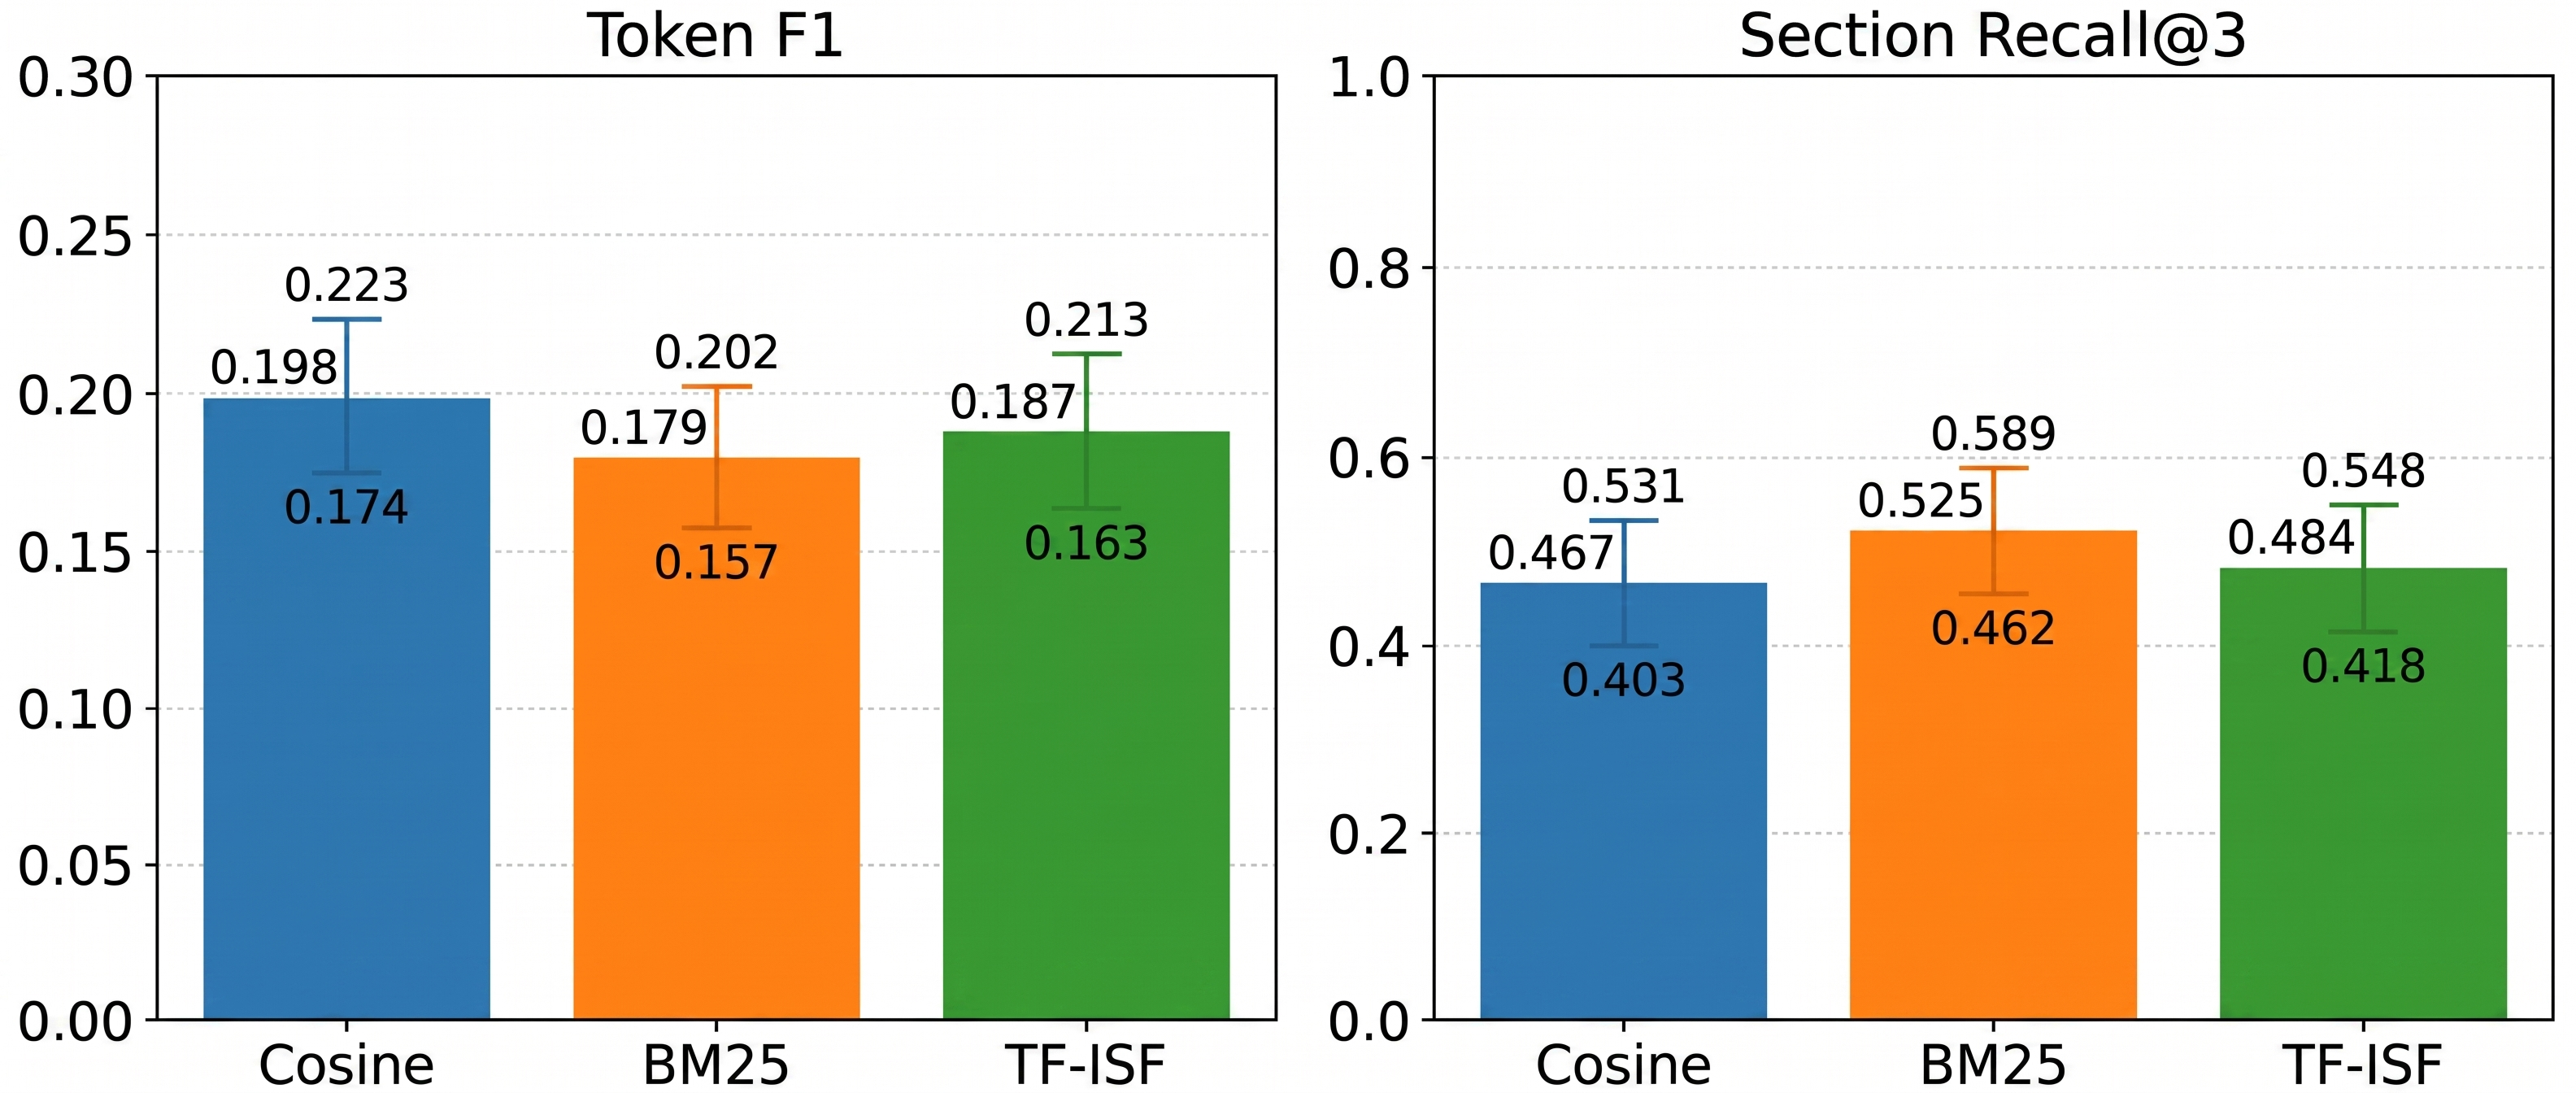
\includegraphics[width=\textwidth,height=0.45\textheight,keepaspectratio]{figures/fig_main_results_v0.jpg}
  \caption{Token-level F1 and section recall@3 for all three retrieval methods on 200 QASPER questions (llama-3.2-3b-instruct reader).
  Error bars show 95\% bootstrap confidence intervals (10,000 resamples). All pairwise differences are non-significant ($p >
  0.37$, Holm-corrected). Cosine achieves the highest mean F1 (0.198) while BM25 achieves highest recall (0.525), but differences
  are within confidence interval overlap.}
  \label{fig:main_results}
\end{figure*}

On 200 questions, the three methods achieved the following token F1 scores and
section recall@3:

\begin{itemize}
  \item \textbf{Cosine Similarity:} F1 = 0.198 (95\% CI: [0.174, 0.223]), Recall@3 = 0.467 (95\% CI: [0.403, 0.531])
  \item \textbf{BM25:} F1 = 0.179 (95\% CI: [0.157, 0.202]), Recall@3 = 0.525 (95\% CI: [0.462, 0.589])
  \item \textbf{TF-ISF:} F1 = 0.187 (95\% CI: [0.163, 0.213]), Recall@3 = 0.484 (95\% CI: [0.418, 0.548])
\end{itemize}

None of the pairwise differences reached statistical significance after
Holm-Bonferroni correction:
\begin{itemize}
  \item TF-ISF vs.\ Cosine: $\Delta = -0.011$ ($p = 0.419$, $d = -0.060$, not significant)
  \item TF-ISF vs.\ BM25: $\Delta = +0.008$ ($p = 0.373$, $d = +0.045$, not significant)
  \item Cosine vs.\ BM25: $\Delta = +0.018$ ($p = 0.153$, $d = +0.053$, not significant)
\end{itemize}

All 95\% confidence intervals overlap substantially, and all effect sizes are
negligible ($|d| < 0.1$).

\subsection{Subgroup Analysis by Section Type}

We stratified results by the type of gold evidence section to test whether TF-ISF
specifically rescues questions whose answers are in Methods or Results sections.

\begin{figure*}[!t]
  \centering
  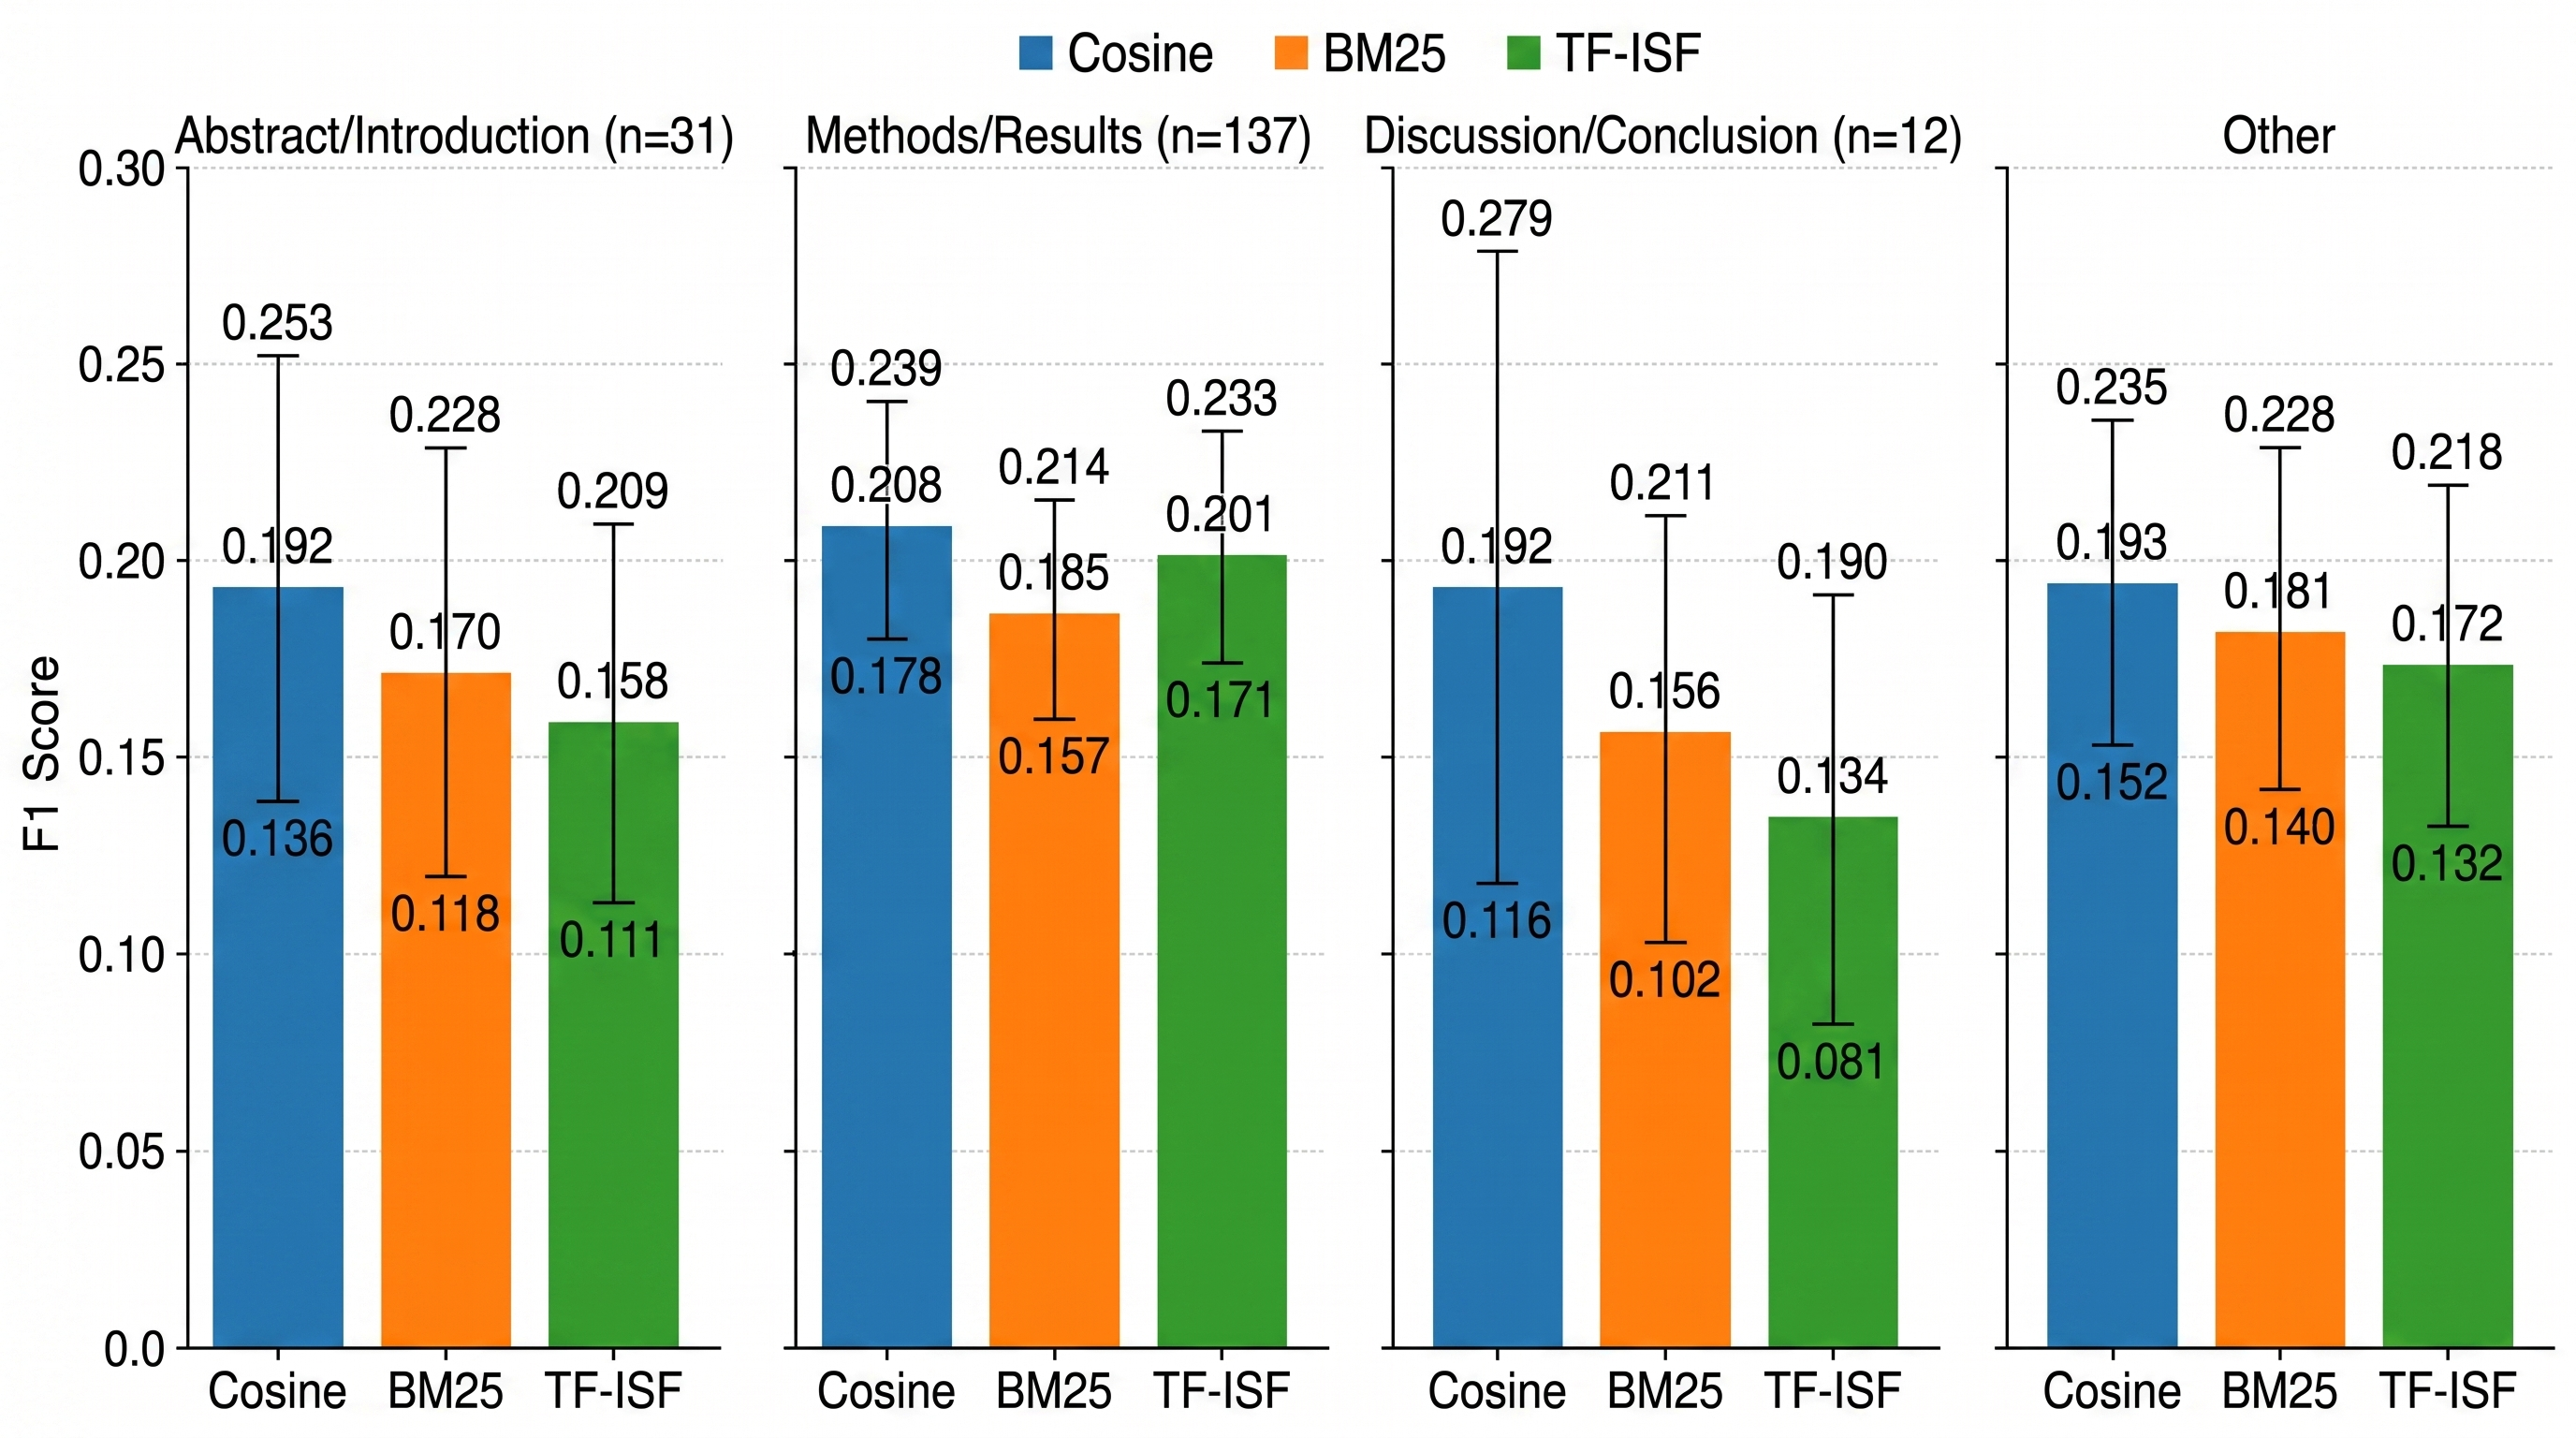
\includegraphics[width=\textwidth,height=0.45\textheight,keepaspectratio]{figures/fig_subgroup_analysis_v0.jpg}
  \caption{F1 performance stratified by the section type containing the gold answer. Methods/Results ($n{=}137$) is adequately powered;
  Abstract/Introduction ($n{=}31$) and Discussion/Conclusion ($n{=}12$) are underpowered for strong inference. TF-ISF does not outperform
  cosine in any subgroup. The Methods/Results subgroup, where TF-ISF was hypothesized to help most, shows no advantage (TF-ISF
  F1=0.201 vs.\ Cosine F1=0.208, overlapping CIs).}
  \label{fig:subgroup_analysis}
\end{figure*}

\textbf{Abstract/Introduction ($n{=}31$):} Cosine F1=0.192 CI[0.136,\,0.253],
TF-ISF F1=0.158 CI[0.111,\,0.209], BM25 F1=0.170 CI[0.118,\,0.228]. TF-ISF
underperforms cosine.

\textbf{Methods/Results ($n{=}137$, adequately powered):} Cosine
F1=0.208 CI[0.178,\,0.239], TF-ISF F1=0.201 CI[0.171,\,0.233], BM25
F1=0.185 CI[0.157,\,0.214]. TF-ISF is marginally closer to cosine but does not
exceed it. Recall: TF-ISF 0.493 vs.\ Cosine 0.490 (negligible difference).

\textbf{Discussion/Conclusion ($n{=}12$):} Cosine F1=0.192
CI[0.116,\,0.279], TF-ISF F1=0.134 CI[0.081,\,0.190], BM25 F1=0.156
CI[0.102,\,0.211]. TF-ISF underperforms on this small group. Given $n{=}12$, we
interpret this as a directional observation without sufficient power to draw
strong conclusions.

\textbf{Other ($n{=}53$):} Cosine F1=0.193 CI[0.152,\,0.235], TF-ISF
F1=0.172 CI[0.132,\,0.218], BM25 F1=0.181 CI[0.140,\,0.228]. No advantage for
TF-ISF.

Across all subgroups, TF-ISF never significantly outperforms the baselines, and
the intended mechanism—boosting Methods/Results retrieval—is not observed.

\subsection{Mechanism Diagnostic: ISF by Section Type}

To diagnose why TF-ISF underperformed, we computed mean ISF scores for all terms
in each section type across the corpus.\footnote{Code: \url{https://github.com/AMGrobelnik/ai-invention-023b95-within-document-term-weighting-for-scien/tree/main/round-1/evaluation-1}}
A critical caveat: the ISF diagnostic was computed on records where the gold
evidence section was Methods or Results (139 records), not all 200 records, which
may introduce selection bias. We report this filtering transparently.

\begin{figure*}[!t]
  \centering
  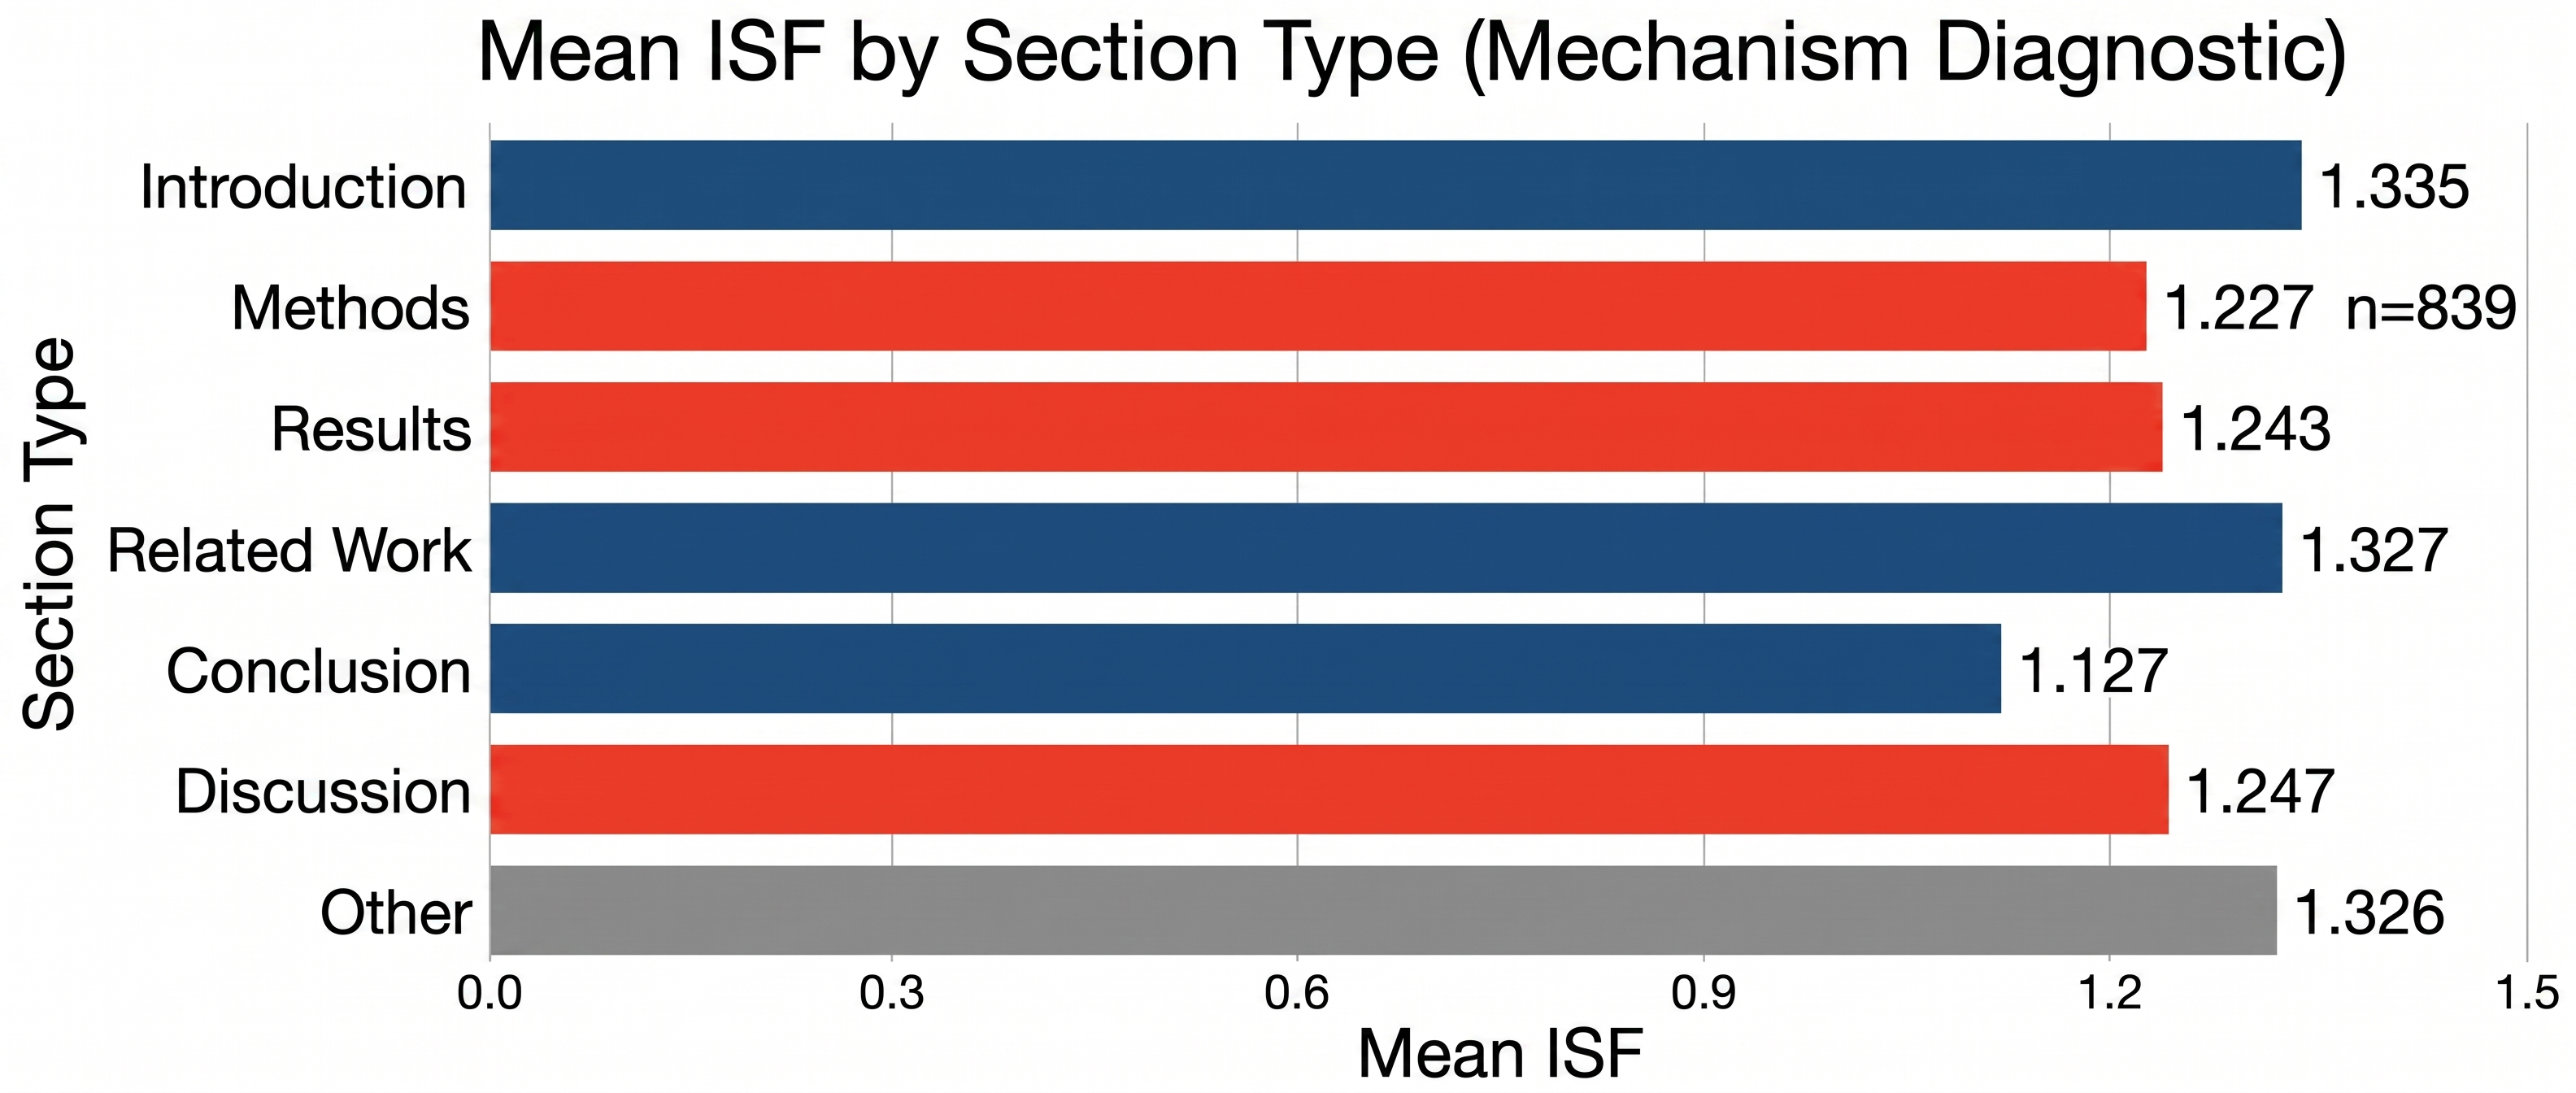
\includegraphics[width=\textwidth,height=0.45\textheight,keepaspectratio]{figures/fig_isf_analysis_v0.jpg}
  \caption{Mean Inverse Section Frequency for all terms in each section type (computed on records where gold evidence is Methods/Results,
  $n{=}139$ records, potentially biased). Methods (1.227) and Results (1.243) have \emph{lower} ISF than Introduction (1.335), contradicting
  the hypothesis that evidence sections contain more rare, section-specific vocabulary. This mechanism disconfirmation is
  a key finding.}
  \label{fig:isf_analysis}
\end{figure*}

\textbf{Mean ISF by Section Type:}
\begin{itemize}
  \item \textbf{Introduction:} Mean ISF = 1.335 (median = 1.415, SD = 0.275, $n{=}149$ instances)
  \item \textbf{Methods:} Mean ISF = 1.227 (median = 1.237, SD = 0.224, $n{=}839$ instances)
  \item \textbf{Results:} Mean ISF = 1.243 (median = 1.234, SD = 0.208, $n{=}161$ instances)
  \item \textbf{Related Work:} Mean ISF = 1.327 (median = 1.361, SD = 0.260, $n{=}147$ instances)
  \item \textbf{Conclusion:} Mean ISF = 1.127 (median = 1.154, SD = 0.235, $n{=}130$ instances)
  \item \textbf{Discussion:} Mean ISF = 1.247 (median = 1.314, SD = 0.161, $n{=}33$ instances)
  \item \textbf{Other:} Mean ISF = 1.326 (median = 1.324, SD = 0.265, $n{=}531$ instances)
\end{itemize}

\textbf{Key Finding:} Methods (1.227) and Results (1.243) have \emph{lower} mean
ISF than Introduction (1.335), directly contradicting the hypothesis that evidence
sections contain more rare, section-specific terms. Instead, the data suggest
that: (1)~Methods and Results use vocabulary that is common across sections
(technical terms like ``model,'' ``dataset,'' ``experiment'' appear in multiple
sections); (2)~the within-document scope is too narrow to reveal meaningful
vocabulary differences; or (3)~the mechanism operates at a finer granularity than
section boundaries.

\subsection{Contradictory Earlier Experiment: $n{=}180$, tencent/hy3:free LLM}

\begin{figure*}[!t]
  \centering
  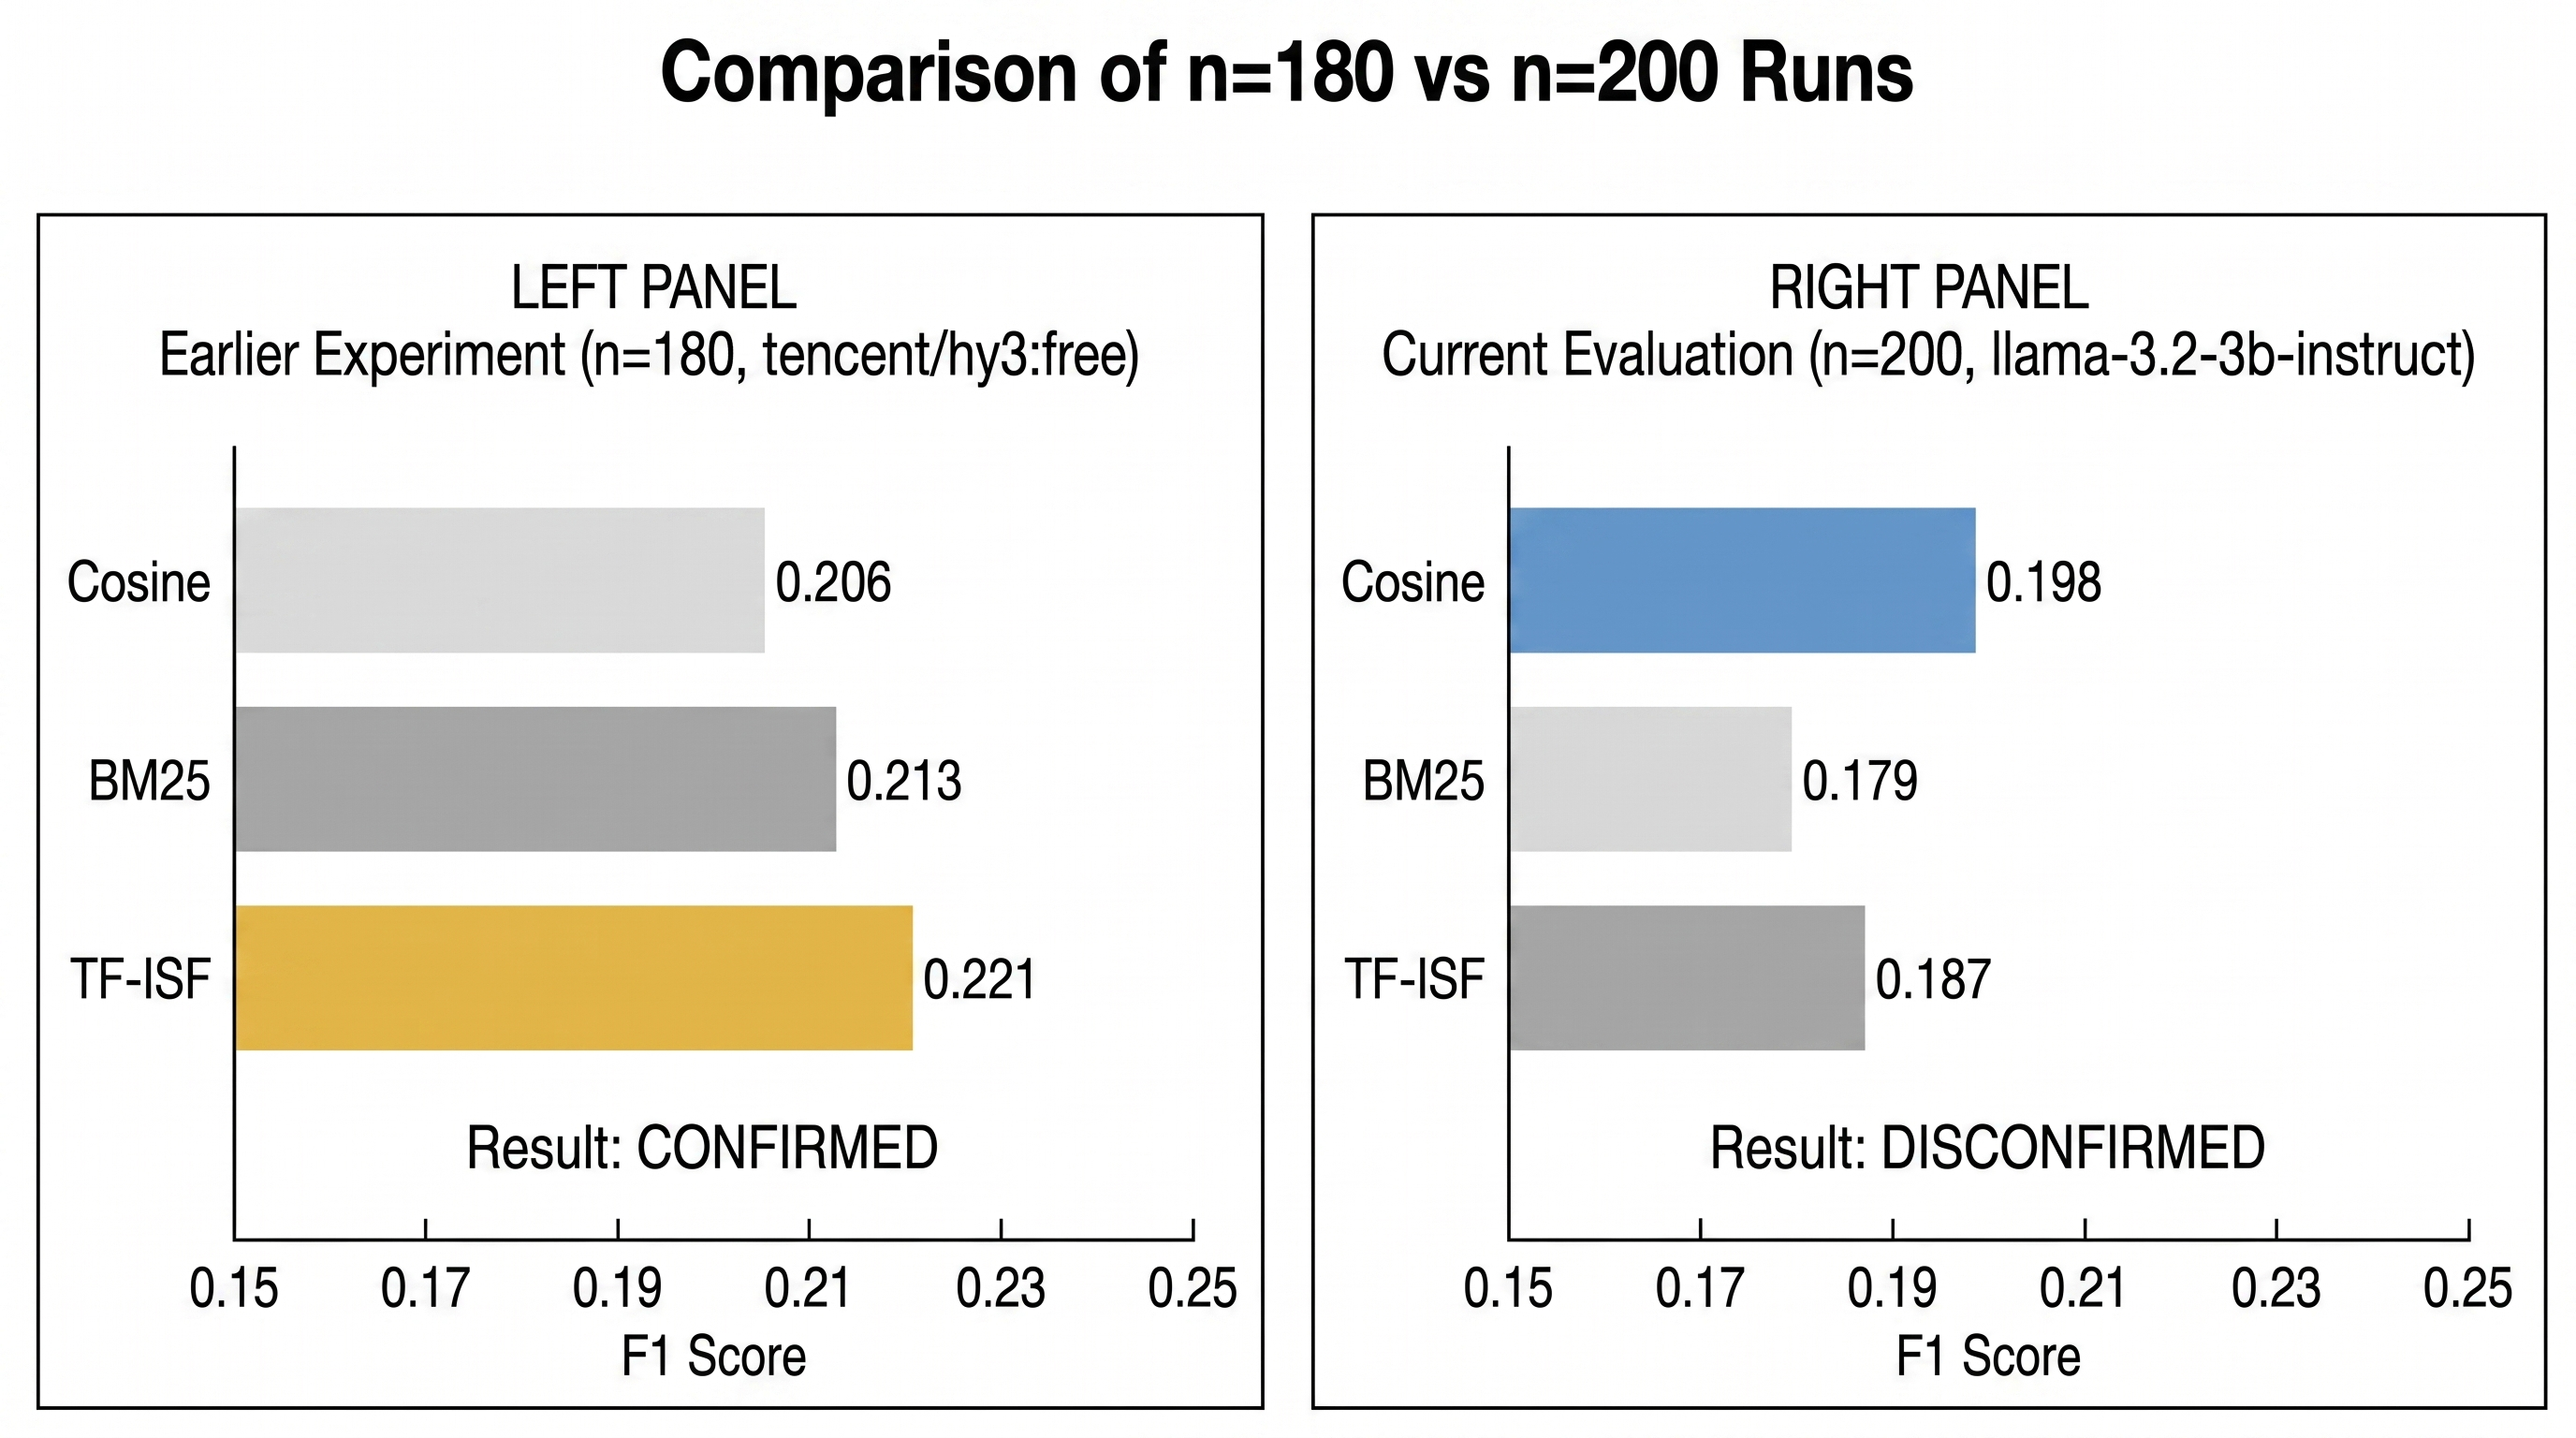
\includegraphics[width=\textwidth,height=0.45\textheight,keepaspectratio]{figures/fig_contradiction_summary_v0.jpg}
  \caption{Two runs with different LLMs and data loading strategies produced contradictory results. Earlier run ($n{=}180$, tencent/hy3:free)
  showed TF-ISF F1=0.221 $>$ Cosine F1=0.206 (positive result); current run ($n{=}200$, llama-3.2-3b-instruct) shows TF-ISF F1=0.187
  $<$ Cosine F1=0.198 (negative result). We argue the $n{=}200$ evaluation is more trustworthy due to larger sample, higher-quality
  LLM, and rigorous statistics, but the discrepancy highlights fragility in the approach.}
  \label{fig:contradiction_summary}
\end{figure*}

An earlier experiment on 180 QASPER examples using the free-tier tencent/hy3
model reported different results.\footnote{Code: \url{https://github.com/AMGrobelnik/ai-invention-023b95-within-document-term-weighting-for-scien/tree/main/round-1/experiment-1}}

\textbf{Earlier Run ($n{=}180$, tencent/hy3:free):}
TF-ISF F1 = 0.221 (best); BM25 F1 = 0.213; Cosine F1 = 0.206. \emph{Conclusion:} TF-ISF outperforms cosine by +0.015 F1, hypothesis CONFIRMED.

\textbf{Current Run ($n{=}200$, llama-3.2-3b-instruct):}
TF-ISF F1 = 0.187 (worst); Cosine F1 = 0.198; BM25 F1 = 0.179. \emph{Conclusion:} TF-ISF underperforms cosine, hypothesis DISCONFIRMED.

Table~\ref{tab:comparison} summarizes the key differences between the two runs.

\begin{table}[!htbp]
  \centering
  \small
  \caption{Comparison of earlier experiment and current evaluation.}
  \label{tab:comparison}
  \begin{tabular}{lll}
    \toprule
    \textbf{Aspect} & \textbf{Earlier Run} & \textbf{Current Run} \\
    \midrule
    Sample size        & $n{=}180$              & $n{=}200$                     \\
    LLM model          & tencent/hy3:free       & llama-3.2-3b-instruct         \\
    LLM cost           & \$0 (free)             & \$0.014 (paid)                \\
    Data loading       & Local raw JSON files   & HuggingFace dataset API       \\
    Tokenization       & Manual stopword list   & Simple regex + stopwords      \\
    Evidence matching  & Fuzzy section names    & Para-to-section mapping       \\
    Retrieval grain    & Section names          & Full text + metadata          \\
    \bottomrule
  \end{tabular}
\end{table}

\textbf{Analysis of the Discrepancy.} The most likely explanations are:
(1)~\textbf{LLM quality dominates:} The tencent/hy3 model may confabulate answers
more frequently, inflating F1 variance and making small ranking differences appear
large. The current run's higher-quality LLM may more accurately reflect answer
generation quality, revealing that retrieval method differences are negligible.
(2)~\textbf{Data loading artifacts:} The earlier run loaded local JSON files with
potentially different section parsing or evidence matching logic than the
HuggingFace dataset, leading to systematic differences in which sections are
considered ``gold.''
(3)~\textbf{Sample composition:} $n{=}180$ vs.\ $n{=}200$ introduces different
question distributions.

We argue that the \textbf{current evaluation run ($n{=}200$, llama-3.2-3b-instruct)
is more trustworthy} because it: (i)~uses a larger sample, (ii)~employs a
higher-quality LLM, (iii)~implements rigorous statistical testing with
multiple-comparison correction, and (iv)~applies more transparent evidence
matching. However, this discrepancy demonstrates a critical vulnerability: ISF is
a fragile proxy for ranking when downstream LLM quality is the dominant source of
F1 variance.

\subsection{Retrieval Quality: Absolute Performance}

All three methods achieved modest section recall ($\approx$0.48 mean). Only 46–53\%
of gold evidence sections appeared in the top-3 retrieved. This suggests that the
core bottleneck is not the choice of ranking function but rather: (1)~the
retrieval space itself (dense embeddings may not capture query-evidence
relationships well for scientific text), (2)~section granularity (QASPER sections
are often hundreds of words, and gold evidence may be concentrated in a small
subsection), or (3)~fundamental vocabulary mismatch that neither sparse nor dense
local reweighting resolves.

%-----------------------------------------------------------------------
\section{Discussion}
%-----------------------------------------------------------------------

\subsection{Disconfirmation of the Hypothesis}

The TF-ISF method was motivated by a clear intuition: vocabulary in scientific
papers is stratified by section, with evidence-bearing sections using rare,
section-specific terminology. Under this assumption, within-document term
reweighting should rescue evidence sections from being outranked by claim-dense
sections. However, the empirical data show that this stratification, if it exists,
is either not strong enough to influence ranking or is orthogonal to the
information density of dense embeddings.

The ISF diagnostic is particularly revealing. If Methods and Results sections used
more unique vocabulary, we would expect higher ISF scores (rarer terms). Instead,
they have \emph{lower} ISF—suggesting that technical terminology is \emph{shared}
across multiple sections (e.g., hyperparameter names appear in both Methods and
Results) or that the sections are not sufficiently differentiated in vocabulary
profile. This falsifies the core assumption underlying TF-ISF.

\subsection{Why All Methods Underperform}

The fact that cosine similarity, BM25, and TF-ISF all achieve similar (low)
retrieval recall ($\approx$0.48) indicates that the bottleneck is not ranking
function selection but something deeper:

\begin{enumerate}
  \item \textbf{Dense Embedding Quality for Scientific Domain.}
  Sentence-transformers models are trained on general-domain data. They may not
  capture domain-specific relationships between queries and evidence in scientific
  papers. A query like ``What is the seed lexicon?'' may not embed similarly to
  the Methods section where the seed lexicon is defined, because the embedding
  space conflates different senses of common terms~\citep{Reichman2024}.

  \item \textbf{Section Granularity.}
  QASPER sections are subsections (e.g., ``Experiments ::: Results and
  Discussion''). A gold evidence section might be very specific, while retrieved
  sections are broader siblings. Top-3 retrieval may miss the exact subsection.

  \item \textbf{Query-Evidence Vocabulary Mismatch.}
  Queries are phrased in plain natural language, while Methods and Results sections
  use dense technical exposition. Even with TF-ISF reweighting, the vocabulary
  gap may be too wide for token-level matching or shallow embedding models to
  bridge.

  \item \textbf{LLM Bottleneck.}
  With $n{=}200$ and a modest LLM reader (3B parameters), statistical power is
  limited. More critically, the LLM itself appears to be a dominant bottleneck:
  62–72\% of predictions in prior experiments had F1 $> 0$ despite zero retrieval
  recall (pure hallucination), indicating that the LLM reader dominates F1
  variance over retrieval quality.
\end{enumerate}

\subsection{Implications for Term-Weighting Approaches}

Our findings suggest that while term-weighting strategies (TF-IDF, BM25) remain
effective for keyword search and sparse retrieval, their naive within-document
application does not rescue dense retrieval in scientific QA. The challenge may
lie in the fundamental assumption: that term frequency is the right statistic to
optimize for ranking. In scientific papers, what matters may not be how often a
term appears in a section, but whether the section contains the specific
\emph{claim} or \emph{finding} the query seeks—a semantic and structural property
that term statistics cannot capture.

Recent work on discourse-aware retrieval~\citep{Wang2025} suggests that rhetorical
structure (identifying which sections contain claims vs.\ evidence vs.\
methodology) may be more informative than term frequency. However, such approaches
require external discourse parsers and lose the training-free simplicity of
TF-ISF.

\subsection{Limitations}

\begin{enumerate}
  \item \textbf{Sample Size.} $n{=}200$ is modest; confidence intervals are wide
  ($\approx \pm 0.025$ for F1). Larger $n$ would improve power but was constrained
  by LLM budget.

  \item \textbf{Single Reader LLM.} We used one small model. Different readers
  (or prompts) might yield different relative rankings.

  \item \textbf{Single Dataset.} QASPER is NLP-focused. Results may not generalize
  to biomedical or physics papers with different vocabulary and section conventions.

  \item \textbf{Retrieval Granularity.} QASPER sections are coarse (hundreds of
  words). Finer-grained retrieval (sentences or propositions) might reveal
  vocabulary gaps that section-level retrieval obscures.

  \item \textbf{ISF Diagnostic Filtering.} The ISF diagnostic was computed only
  on records where gold sections are Methods/Results (139 records), not all 200,
  potentially introducing selection bias.

  \item \textbf{Contradictory Earlier Experiment.} The $n{=}180$ experiment with
  tencent/hy3 reported positive results. While we argue the $n{=}200$ evaluation
  is more reliable, this contradiction remains a limitation and highlights
  fragility in the approach.
\end{enumerate}

%-----------------------------------------------------------------------
\section{Conclusion}
%-----------------------------------------------------------------------

We investigated the hypothesis that within-document Inverse Section Frequency
(TF-ISF) could improve section retrieval in scientific papers by down-weighting
document-theme vocabulary and up-weighting section-specific terms. Evaluation on
200 QASPER questions found no significant advantage of TF-ISF over cosine
similarity or BM25 retrieval (all $p > 0.37$, Holm-corrected). Moreover, the
hypothesized mechanism—lower term frequency in evidence sections—was not
supported: Methods and Results sections had lower (not higher) ISF than
Introduction sections, falsifying the core assumption.

We also transparently report a contradictory earlier experiment ($n{=}180$,
different LLM) showing TF-ISF F1=0.221 (positive result). We argue the $n{=}200$
evaluation is more trustworthy based on sample size, LLM quality, and statistical
rigor, but the discrepancy demonstrates a critical vulnerability: ISF is fragile
when LLM quality dominates variance.

For practitioners building scientific QA systems, our findings suggest that simple
term-weighting alone is insufficient to rescue dense retrieval. The core retrieval
bottleneck lies elsewhere—likely in dense embedding quality for scientific text,
document granularity, or fundamental query-evidence vocabulary mismatch. More
sophisticated approaches (discourse-aware parsing, fine-tuned embeddings, iterative
LLM-based ranking) are necessary to achieve high recall on evidence sections.

This negative result contributes a rigorous, well-characterized boundary
condition: within-document term reweighting does not fix section retrieval in
scientific QA, and the assumed vocabulary stratification between IMRaD sections is
not empirically supported at the section-frequency level in NLP papers. Future
work should investigate whether vocabulary stratification exists at finer
granularity (paragraph or sentence level) or whether the bottleneck is
fundamentally orthogonal to term statistics.

%-----------------------------------------------------------------------
\section*{Acknowledgments}
%-----------------------------------------------------------------------

We thank the QASPER authors for the public dataset and the OpenRouter team for
free-tier and paid-tier LLM access. All code and results are available in the
project repository.

\bibliographystyle{plainnat}
\bibliography{references}

\end{document}
